\documentclass[12pt]{article}
\usepackage[a4paper, margin=1in]{geometry}
\usepackage[T1]{fontenc}
\usepackage{graphicx} % Required for inserting images
\usepackage[backend=bibtex]{biblatex}
\usepackage{hyperref}
\usepackage{dirtree}
\usepackage{textcomp}
\usepackage{listings}
\usepackage{xcolor}
\usepackage{booktabs}
\usepackage{tabularx}
\lstset{basicstyle=\ttfamily\small, columns=fullflexible, keepspaces=true, frame=single,
        backgroundcolor=\color{gray!8}, rulecolor=\color{gray!40}, xleftmargin=0.5em, xrightmargin=0.5em,
        aboveskip=0.6em, belowskip=0.6em, showstringspaces=false, upquote=true}
\title{\textbf{Mini Game Hub}}
\author{Larissa \\ Sahil Deo}
\date{\today}
\addbibresource{references.bib}
\begin{document}
\maketitle
\tableofcontents
\clearpage
\section{Security: Bash-Specific Vulnerabilities in Authentication}

The login in \texttt{main.sh} reads untrusted text from the keyboard and splices it into \texttt{grep} and \texttt{sed} patterns and into the tab- and comma-separated files that store accounts and lockouts. Bash has several quirks that turn this kind of code into a security problem: it can silently rewrite input, treat data as command options, or treat data as a pattern. This section lists each risk we considered, how the code deals with it, and one rare bug we found and fixed while reviewing our own code.

\subsection{Option injection into \texttt{echo} (found and fixed)}
Passwords were hashed with
\begin{lstlisting}
hash(){ echo -n "$@" | sha256sum | cut -d ' ' -f 1; }
\end{lstlisting}
The \texttt{-n} was there to stop \texttt{echo} adding a trailing newline, which would change the hash. The flaw is that Bash's \texttt{echo} does not accept \texttt{-{}-} to end its options, so it reads its \emph{argument} as more options whenever that argument looks like one \cite{bash_builtins}. A password of \texttt{-n}, \texttt{-e} or \texttt{-E} (or combinations such as \texttt{-ne}) is swallowed as a flag, nothing is printed, and the password is stored as the SHA-256 hash of the \emph{empty string}:
\begin{lstlisting}
$ echo -n "-n" | sha256sum      # e3b0c442...  (same as the empty string)
$ echo -n ""   | sha256sum      # e3b0c442...
$ printf '%s' "-n" | sha256sum  # 5249f4fc...  (correct)
\end{lstlisting}
Two things go wrong. All of these passwords collide with each other, and an account whose password is \texttt{-n} can be entered by pressing Enter at the password prompt. The fix is to print with \texttt{printf}, whose format string is fixed, so the password is only ever data:
\begin{lstlisting}
hash(){ printf '%s' "$*" | sha256sum | cut -d ' ' -f 1; }
\end{lstlisting}

\subsection{Input that \texttt{read} silently rewrites}
\begin{itemize}
    \item \textbf{Backslashes.} Plain \texttt{read} treats a backslash as an escape character and deletes it, so the password \texttt{a\textbackslash b} would be stored as \texttt{ab}. Every \texttt{read} uses \texttt{-r}, which keeps backslashes literal.
    \item \textbf{Leading and trailing spaces (fixed).} Even with \texttt{-r}, \texttt{read} trims leading and trailing spaces and tabs using \texttt{IFS}, so \texttt{" pw "} and \texttt{"pw"} were the same password. Password prompts now use \texttt{IFS= read -r -s}, which keeps every character.
    \item \textbf{Echoing.} Passwords are read with \texttt{-s}, so they are never shown on screen.
\end{itemize}

\subsection{Pattern and record injection through usernames}
The username is placed directly inside regular expressions and a \texttt{sed} command:
\begin{lstlisting}
grep -q  "^${name}${tab}"          .user_files/.users.tsv
grep -E  "^${username},[0-9]+$"    .system_files/.failed_logins.csv
sed  -i  "/^$line$/d"              .system_files/.failed_logins.csv
\end{lstlisting}
A username such as \texttt{.*} would match other users' rows, a \texttt{/} would break out of the \texttt{sed} address, and a tab, comma or newline would let a user write forged rows into the account or lockout files. We prevent all of these by accepting only usernames that match \texttt{\^{}[a-zA-Z0-9\_]+\$}. Such a name contains no regex metacharacters, no \texttt{sed} delimiter and none of the file delimiters, so it can be inserted into these patterns safely.

\subsection{Checking the password}
The credential check builds the line \texttt{username<TAB>hash} and looks for it with
\begin{lstlisting}
grep -Fxq "$line" .user_files/.users.tsv
\end{lstlisting}
\texttt{-F} treats the line as a fixed string rather than a regex, and \texttt{-x} requires the whole line to match \cite{grep_manual}, so no partial or prefix match can authenticate a user. Because only the 64-character hexadecimal hash is ever stored or compared, special characters in a password (quotes, backslashes, tabs, \texttt{\$}) can never reach a file or a pattern.

\subsection{Other Bash hazards}
\begin{itemize}
    \item \textbf{Word splitting and globbing.} Every expansion of user input is double-quoted (\texttt{"\$u1"}, \texttt{"\$pwd"}), so a \texttt{*} or a space in input is never expanded into file names or split into several arguments.
    \item \textbf{Passwords in the process list.} \texttt{printf} is a Bash builtin and the password reaches \texttt{sha256sum} through a pipe, so it never appears as a command-line argument visible to other users through \texttt{ps}.
    \item \textbf{Brute force.} After three wrong passwords the account is locked for 60 seconds, with the lock time recorded in \texttt{.system\_files/.failed\_logins.csv}.
\end{itemize}

\subsection{Summary and remaining limitations}
\begin{center}
\small
\begin{tabularx}{\textwidth}{>{\raggedright\arraybackslash}p{4.2cm} >{\raggedright\arraybackslash}X >{\raggedright\arraybackslash}p{3.6cm}}
\toprule
\textbf{Risk} & \textbf{Effect if unhandled} & \textbf{Defence} \\
\midrule
Option injection into \texttt{echo} & Passwords \texttt{-n}, \texttt{-e}, \texttt{-E} hash as the empty string & \texttt{printf '\%s'} (fixed) \\
Backslash escapes in \texttt{read} & Backslashes silently removed & \texttt{read -r} \\
Whitespace trimming in \texttt{read} & Leading/trailing spaces ignored & \texttt{IFS= read -r} (fixed) \\
Regex / \texttt{sed} injection & Matching or deleting other users' rows & Username whitelist \\
Delimiter injection & Forged account or lockout rows & Username whitelist; only hashes stored \\
Partial matches & Logging in on a prefix match & \texttt{grep -Fx} \\
Word splitting, globbing & Input expanded or split & Quoting every expansion \\
Password guessing & Unlimited attempts & 60-second lockout \\
\bottomrule
\end{tabularx}
\end{center}
Two weaknesses remain and are listed under future work: the hashes are unsalted SHA-256, which is fast to brute-force if \texttt{.users.tsv} leaks (a salted, deliberately slow hash such as bcrypt or Argon2 would be better), and the data files are hidden but not protected by file permissions.

\clearpage
\section{External Libraries}
\begin{itemize}
\item \textbf{numpy} - Used for efficient handling of arrays and game board matrix. It simplifies operations on the game board, such as checking valid moves, updating states, and checking the win condition.

\item \textbf{pygame-ce} - Used for building the graphical user interface of the games. It handles rendering, mouse detection, game loops, and animations.

\item \textbf{matplotlib} - Used for visualizing game statistics such as top 5 winners and the frequencies of each game

\item \textbf{time} - Used for implementing delays, timers, and tracking time-based events within games.

\item \textbf{os} - Used for interacting with the file system via bash (os.system())

\item \textbf{sys} - Used for taking command line arguments for game.py 
\end{itemize}

\section{Design \& Architecture}

\subsection{Authentication System (Bash)}
User authentication is handled via shell scripts:
\begin{itemize}
    \item User credentials are stored in \texttt{.users.tsv} with SHA-256 hashed passwords.
    \item Login allows 3 attempts before temporary lockout.
    \item Lockout timestamps are stored in \texttt{.failed\_logins.csv}.
    \item Defences against Bash-specific attacks are described in Section~1.
\end{itemize}

\subsection{Leaderboard System}
Game statistics are stored in CSV files. The leaderboard script:
\begin{itemize}
    \item Sorts users by wins, losses, or win/loss ratio
    \item Formats output using \texttt{column}
    \item Maintains a top-5 players file
\end{itemize}


\subsection{Game Class Abstraction}
The \texttt{Game} class stores:
\begin{itemize}
    \item The board as a NumPy 2D array
    \item Current player turn (boolean)
    \item Board dimensions and cell size
\end{itemize}
It provides utility functions such as \texttt{switchTurn()}, \texttt{valid\_move()}, and a pluggable \texttt{checkWin()} function passed during initialization, allowing reuse across different games.

\subsection{Rendering and Scaling}
All rendering is done using \texttt{pygame}. Custom scaling functions \texttt{scale\_h()} and \texttt{scale\_w()} ensures resolution-independent scaling by mapping coordinates relative to a reference screen size.

Static elements such as boards are pre-rendered onto \texttt{Surface} objects and blitted every frame to improve performance.

\subsection{Event Handling and Game Loop}
Each game runs a main loop that:
\begin{itemize}
    \item Captures user input (mouse clicks, key presses)
    \item Updates game state (moves, turn switching, timers)
    \item Renders updated visuals
\end{itemize}
Mouse clicks are mapped to board cells, and moves are executed only if valid.

\subsection{Win Detection}
Each game defines its own \texttt{checkWin()}:
\begin{itemize}
    \item Tic Tac Toe and Connect 4 scan in 4 directions (horizontal, vertical, both diagonals) using NumPy slicing.
    \item Othello determines the winner by counting pieces when no valid moves remain (using \texttt{np.sum()})
\end{itemize}

\subsection{Animations}
Animations are time-based using timestamps:
\begin{itemize}
    \item Tic Tac Toe: progressive drawing of crosses (line segments) and circles (arc sweep).
    \item Connect 4: falling discs simulated using $y = \frac{1}{2}gt^2$.
    \item Othello: flipping discs using \texttt{pygame.draw.ellipse()} and expansion.
\end{itemize}

Jagged drawing effects are implemented via the \texttt{JaggedLine} class, which perturbs line segments randomly for a hand-drawn aesthetic.
\texttt{pygame.draw.arc()} is naturally jagged, which is what inspired the hand-drawn aesthetic.

\subsection{Blitz Mode}
A \texttt{Timer} class manages turn-based countdowns. Each player’s timer activates only during their turn. The remaining time is displayed as a dynamically coloured vertical bar, transitioning from green to red as time decreases.

\subsection{User Interface Components}
Reusable UI elements include:
\begin{itemize}
    \item \texttt{Button}: handles hover, click feedback, and rendering
    \item \texttt{Box}: used for popups and text displays
\end{itemize}
End-of-game overlays use semi-transparent surfaces to dim the screen and display options like ``Play Again'' and ``Main Menu''.

\subsection{Othello Move Logic}
Valid moves are computed by scanning in all 8 directions from each empty cell. A move is valid if it captures at least one opponent piece bracketed by the current player's pieces. Piece flipping is performed by updating slices of the NumPy array.

\subsection{Connect 4 Mechanics}
Each column tracks the number of filled cells. When a move is made, the disc is placed in the lowest available row. Falling animation is applied until the disc reaches its final position.

\subsection{Flowchart:}

\begin{center}
\begin{tabular}{c}
Start \\
$\downarrow$ \\
Authentication (main.sh) \\
$\downarrow$ \\
Select Game (game.py)\\
$\downarrow$ \\
Choose Time Control (game.py)\\
$\downarrow$ \\
Toss to Decide First Player (game.py)\\
$\downarrow$ \\
\begin{tabular}{ccc}
TicTacToe & Connect4 & Othello \\
play() & play() & play()
\end{tabular} \\
$\downarrow$ \\
Return Result \\
$\downarrow$ \\
Leaderboard (leaderboard.sh) \\
$\downarrow$ \\
End
\end{tabular}
\end{center}

\section{Features Implemented}
    \subsection{Authentication System}
    \begin{itemize}
        \item Supports user registration and login with passwords securely hashed using SHA-256.
        \item Two-player authentication is required before starting a game.
        \item The system enforces a 3-attempt login limit per user, after which a temporary time-based lockout is applied.
    \end{itemize}
    
    \subsection{Blitz Feature}
    \begin{itemize}
        \item A timed gameplay mode where each player must make a move within a specified time limit.
        \item The remaining time is visually represented using a vertical timer bar which changes colour according to the urgency of move.
    \end{itemize}


    \subsection{Animations} Visual enhancements implemented to improve user experience:
    \begin{itemize}
        \item Tic Tac Toe: drawing animations for X and O symbols, along with a line animation highlighting the winning combination.
        \item Othello: coin flipping with a wave-like animation to represent piece conversion visually.
        \item Connect Four: a falling animation for coins to simulate realistic gravity-based placement.
    \end{itemize}

	\subsection{Performance Optimization}
	\begin{itemize}
        \item Using set in Othello to improve performance
		\item Storing data in .user\_files to avoid processing from history.csv everytime - Time complexity improvement from O(nlogn) to O(u), where n is number of games and u is number of users
		\item Preprocessing static images/frames onto Surfaces and only blitting at runtime
    \end{itemize}

    \subsection{Abstractions}
    \begin{itemize}
        
        \item \textbf{Developer Point of View}
            \begin{itemize}
                \item Design elements which are inheritable as a Class Button, Box, Jagged Line etc.
                \item Menus - callable as a function, returns the choice  
                \item Auto-Sizing of Text - Using Binary Search text is automatically fit to Box/Button - we try a font, and get its rect - If it doesn't fit, we try a font size smaller (We do this using binary search between 1 to 100)
             
            \end{itemize}
        \item \textbf{User Point of View}
            \begin{itemize}
                \item GameHub folder is clean - system files and user files are hidden
                \item Intuitive Menus and usage             
            \end{itemize}
       

\end{itemize}


\section{Directory Structure}

\dirtree{%
.1 \texttt{hub/}.
.2 \texttt{main.sh}.
.2 \texttt{game.py}.
.2 \texttt{leaderboard.sh}.
.2 \texttt{reset.sh}.
.2 \texttt{games/}.
.3 \texttt{tictactoe.py}.
.3 \texttt{connect4.py}.
.3 \texttt{othello.py}.
.3 \texttt{classGame.py}.
.3 \texttt{design\_elements.py}.
.2 \texttt{images/}.
.3 \texttt{red\_disc.png}.
.3 \texttt{yellow\_disc.png}.
.2 \texttt{.user\_files/}.
.3 \texttt{.stats\_tictactoe.csv}.
.3 \texttt{.stats\_connect4.csv}.
.3 \texttt{.stats\_othello.csv}.
.3 \texttt{.users.tsv}.
.3 \texttt{.user\_total\_wins.csv}.
.3 \texttt{.history.csv}.
.3 \texttt{.top5.txt}.
.3 \texttt{.game\_frequencies.csv}.
.2 \texttt{.system\_files/}.
.3 \texttt{.failed\_logins.csv}.
.2 \texttt{report/}.
.3 \texttt{report.tex}.
.3 \texttt{report.pdf}.
.3 \texttt{references.bib}.
.3 \texttt{makefile}.
.3 \texttt{images/}.
}

\section{Installation \& Setup}
\begin{verbatim}
pip install numpy pygame-ce matplotlib
\end{verbatim}

\section{Usage}

Run the main script to start the application:
\begin{verbatim}
bash main.sh
\end{verbatim}

\subsection*{Authentication}
Two users are prompted to log in via the terminal. Each user has up to three attempts before a temporary lockout.

\begin{center}
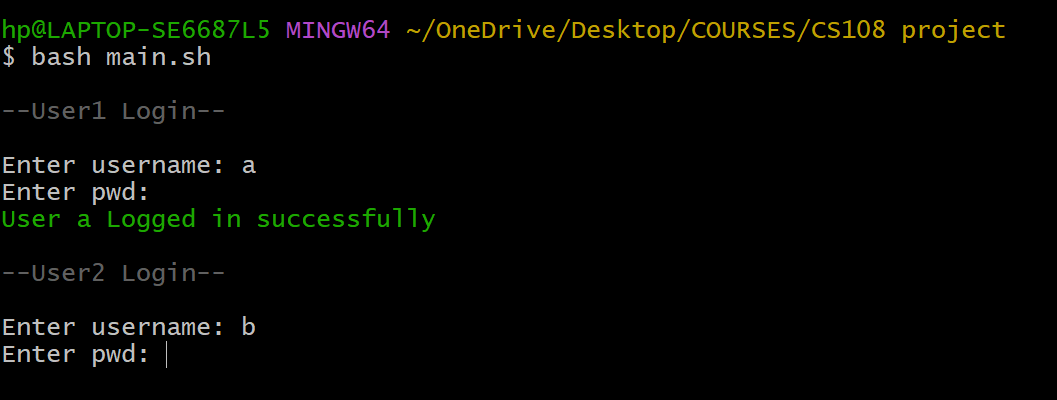
\includegraphics[width=0.6\textwidth]{images/use_main.sh.png}
\end{center}

\subsection*{Main Menu}
After launching, the main menu is displayed with options to start a game or view the leaderboard.

\begin{center}
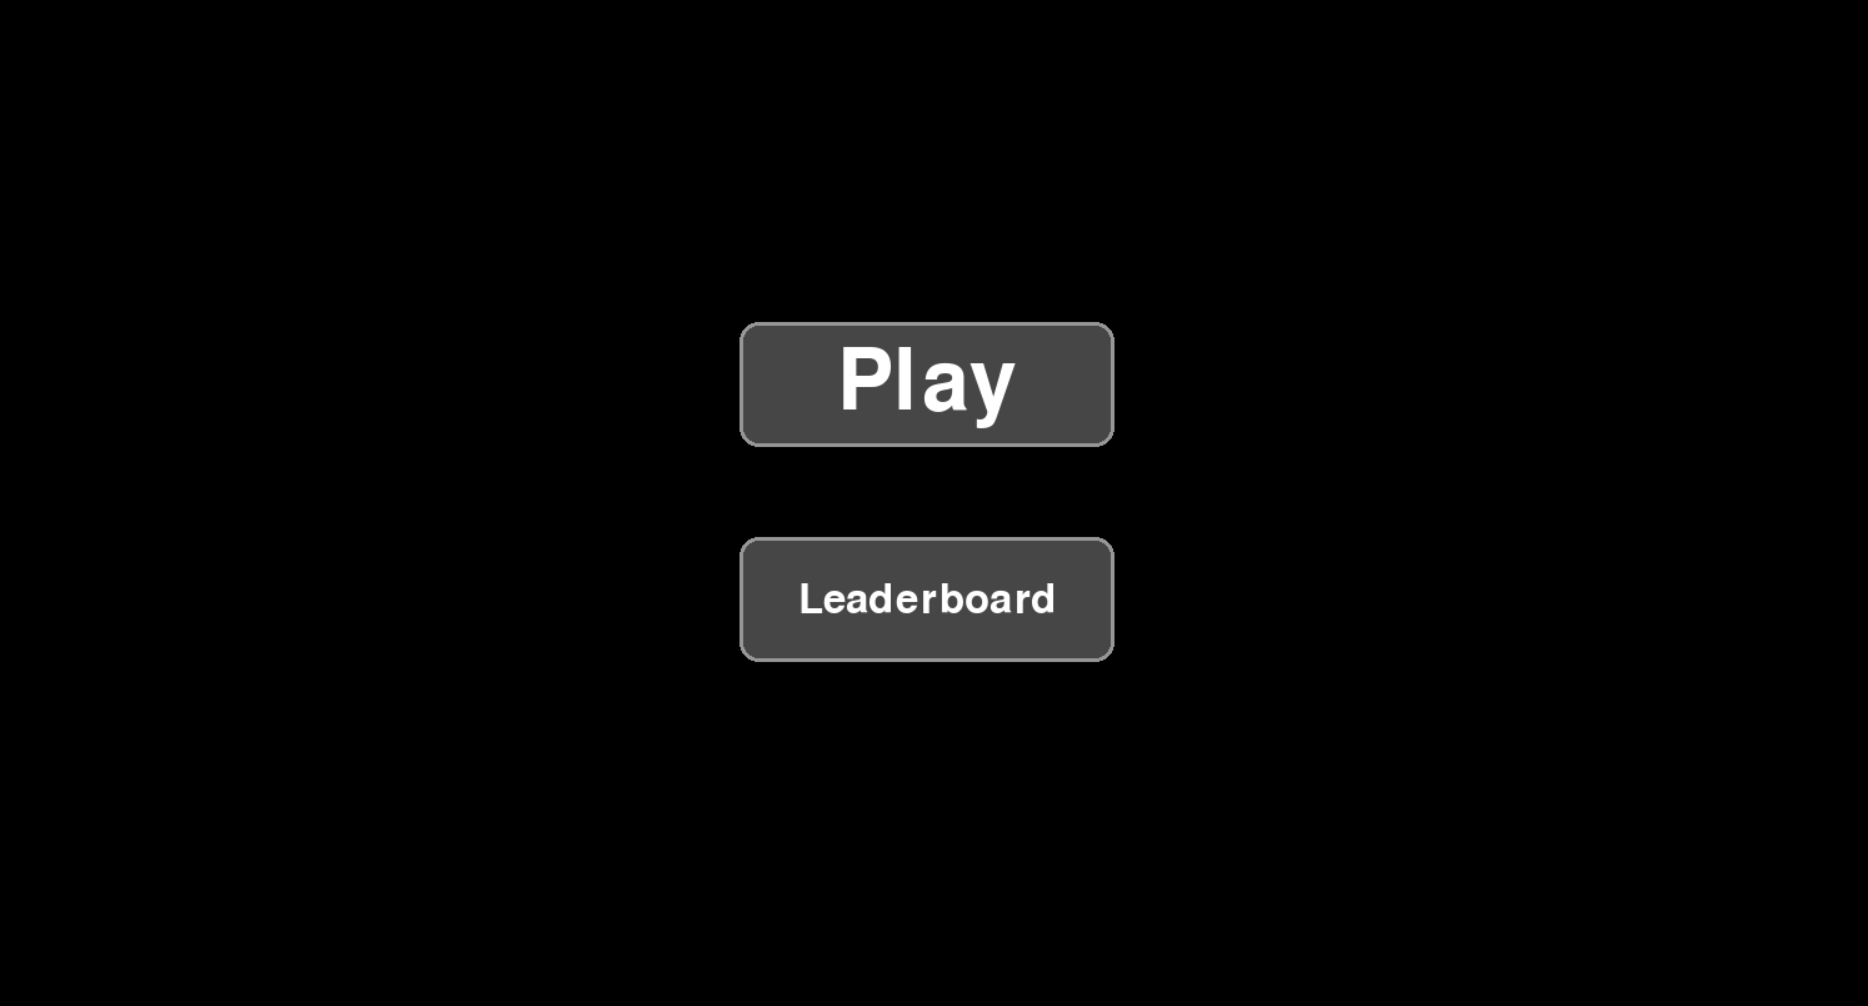
\includegraphics[width=0.6\textwidth]{images/Main_menu.png}
\end{center}

If play is clicked:

\subsection*{Choosing game}
Click the button for game you want

\begin{center}
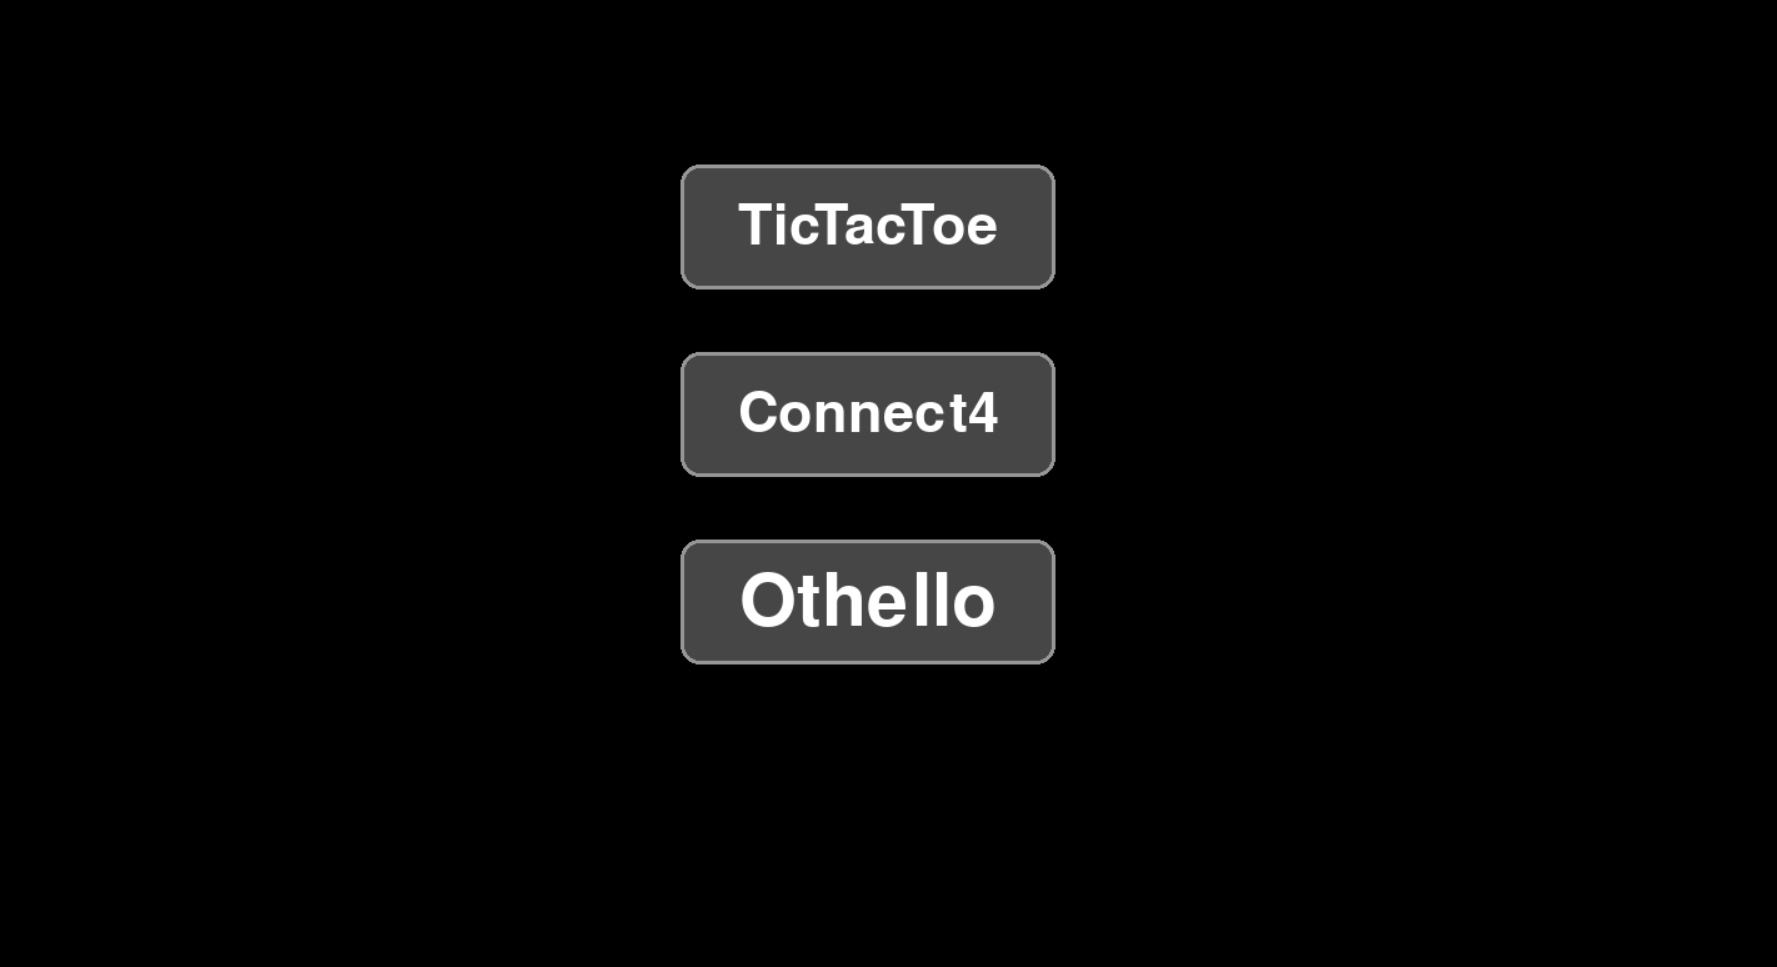
\includegraphics[width=0.6\textwidth]{images/game_menu.png}
\end{center}

\subsection*{Choosing time control}
Click the time control you want

\begin{center}
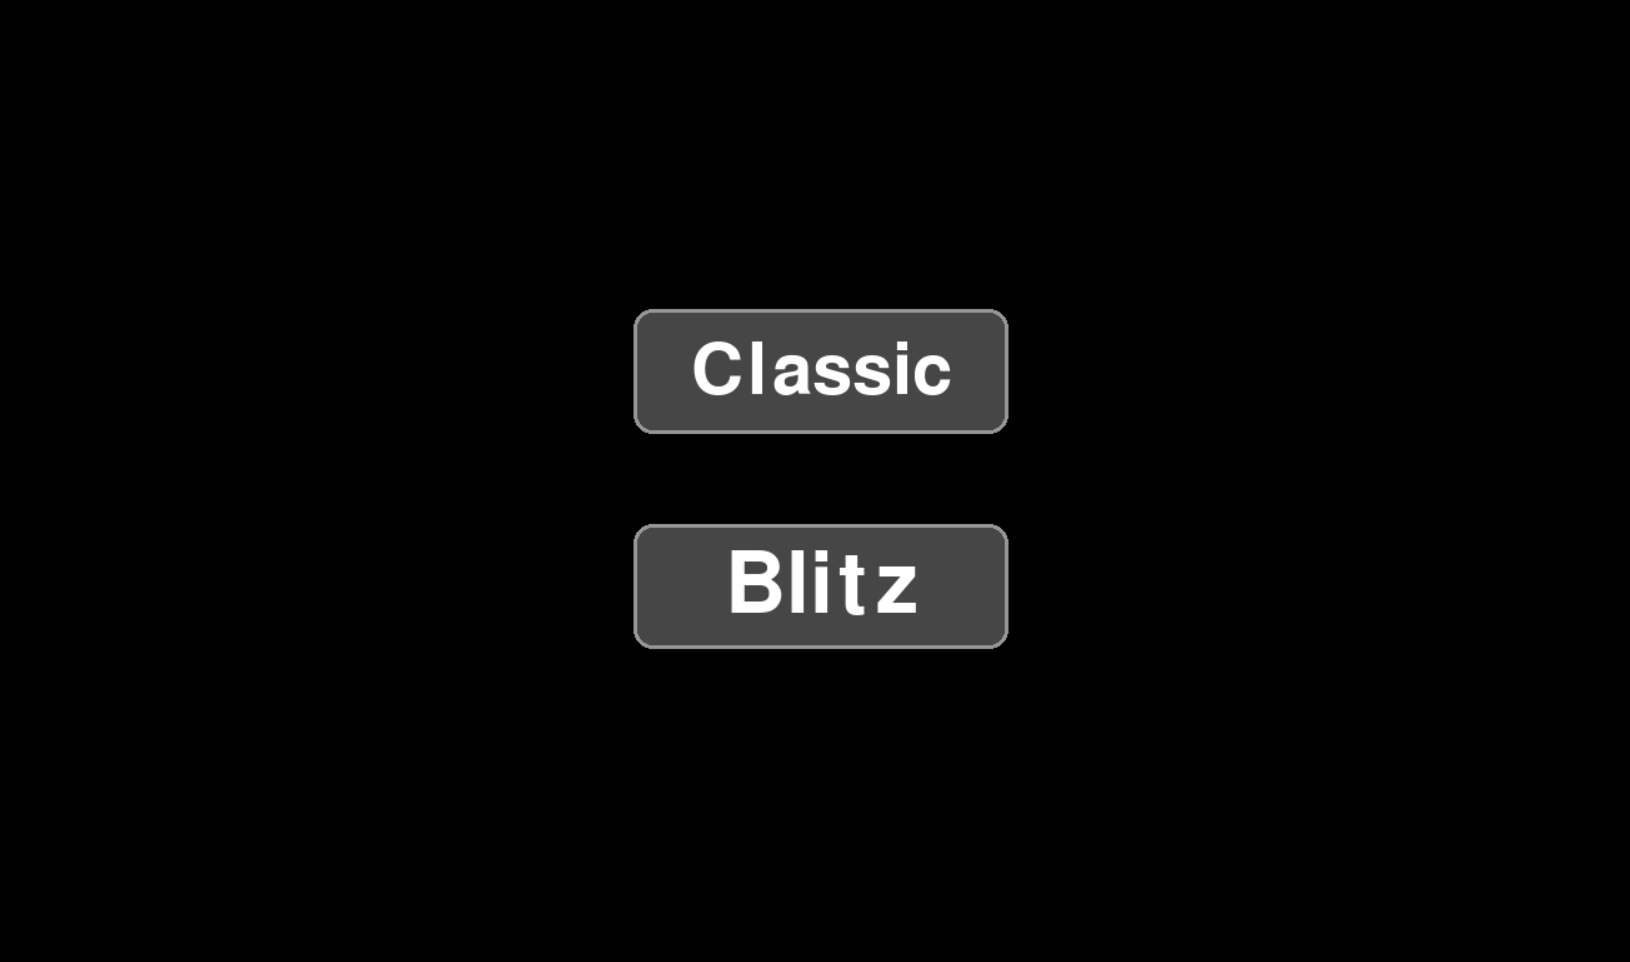
\includegraphics[width=0.6\textwidth]{images/time_menu.png}
\end{center}

\subsection*{Leaderboard Menu}
Click metric to sort by and game name for stats. The first choice is highlighted red until second is chosen
\begin{center}
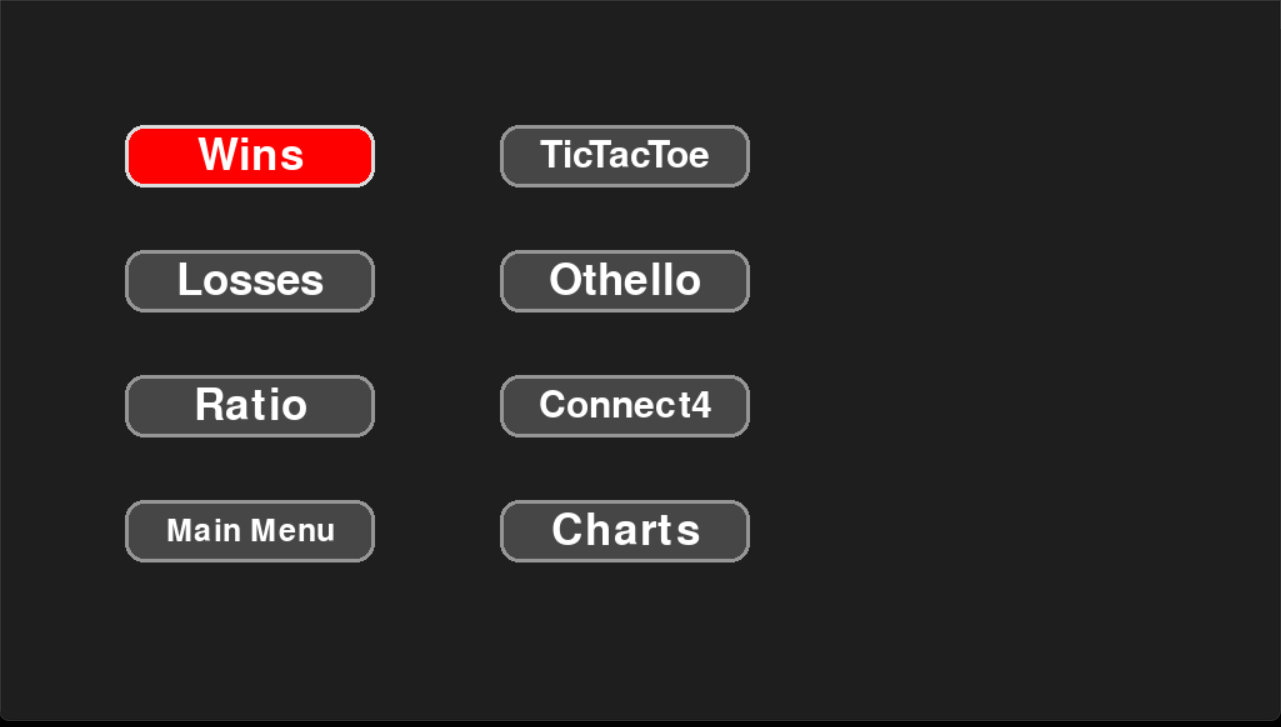
\includegraphics[width=0.6\textwidth]{images/Use_leaderboard.png}
\end{center}

\subsection*{Leaderboard Output}
The leaderboard is displayed in the terminal in a formatted table.

\begin{center}
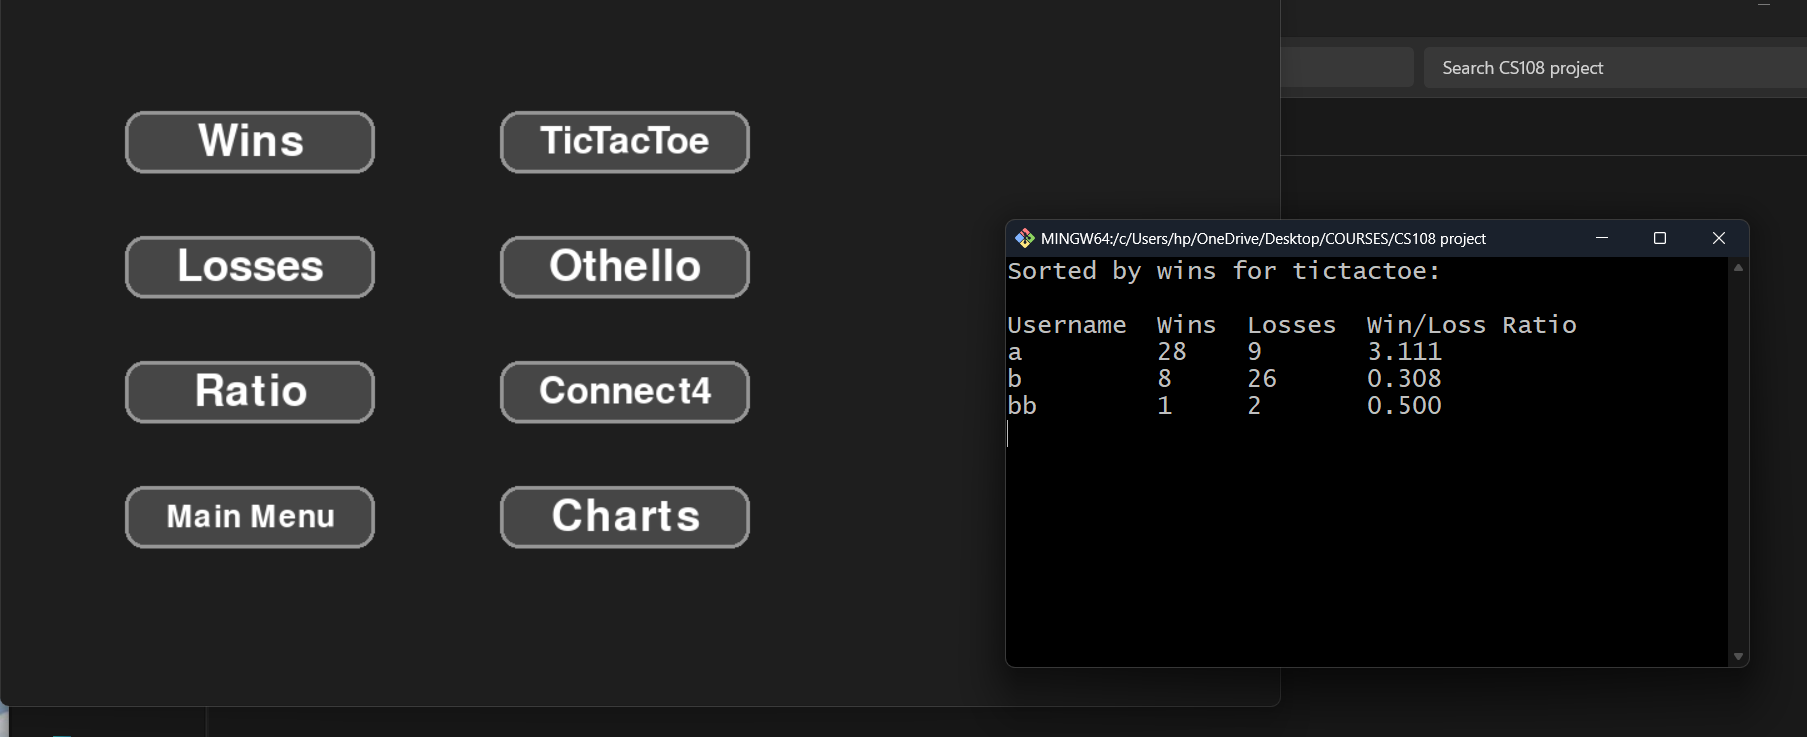
\includegraphics[width=0.6\textwidth]{images/leaderboard_result.png}
\end{center}

\section{Retrospective}
\begin{itemize}
    \item Accidental change of the same part by both teammates - \\
    \emph{Fix:} Clearly communicating beforehand, and also doing a merge commit when necessary
    \item Lagging animation - \\
    \emph{Fix:} Performance improved by precomputing static frames onto Surface objects and then blitting them to the screen at loop runtime \cite{pygame_surface}
    \item Timer and Toss Bar fluid going out of box for low levels - \\
    \emph{Fix:} Using pygame Surfaces transparency feature - made a window Surface \\ which lets viewer peek through only the shape we want, hence clipping the fluid \cite{pygame_transparency}
    \item Scaling of sizes across systems - \\
    \emph{Fix:} Using scaling functions wherever necessary
    \item Not able to change game board values in Othello - the diagonal array extracted from game board using the diagonal() function was not writable by default.\\
    \emph{Fix:} Used arr\_name.setflags(write=1) \cite{numpy_setflags}
    \item Seed was same for all board lines since time was converted to int, and execution was finished in less than a second. \\
    \emph{Fix:} Used int(time\_ns())
    \item Unnecessary complicated scaling by introducing a Size class - \\
    \emph{Fix:} Removed overcomplicated Size class, changed it to simple scaling functions 
    \item Passwords \texttt{-n}, \texttt{-e} and \texttt{-E} were hashed as the empty string, because \texttt{echo -n "\$@"} read them as options - \\
    \emph{Fix:} Hash with \texttt{printf '\%s' "\$*"} instead (Section~1.1) \cite{bash_builtins}
	\item Pygame Events during toss() like random clicks and ESCAPE were getting transferred to next loop - \\
    \emph{Fix:} \texttt{pygame.event.clear()}
\end{itemize}

\section{What we would do differently with 10 more hours}

\subsection{Code Architecture Improvements}
\begin{itemize}
\item Introduce a state-machine type flow for game.py to simplify the logic 
\item Create a Menu Class with Button and Box as subclass
\item Use enums for things like whose turn is it to avoid all the confusion during development
\item Replace unsalted SHA-256 with a salted, slow password hash (bcrypt or Argon2) and restrict permissions on the data files
\end{itemize}

\subsection{User Experience Enhancements}
\begin{itemize}
\item Add smoother scene transitions (fade in/out between menus and games).
\item Improve aesthetics and feedback (hover effects, button animations, sound effects).
\item Add a pause button
\end{itemize}

\subsection{Feature Expansion}
\begin{itemize}
\item Add single-player mode which just chooses random choices (Just for fun)
\item Figure out a cleaner leaderboard display aesthetic so we can see terminal output simultaneously
\item Create a visual interface to choose how many seconds per move in blitz
\end{itemize}

\nocite{*}
\printbibliography
\end{document}
